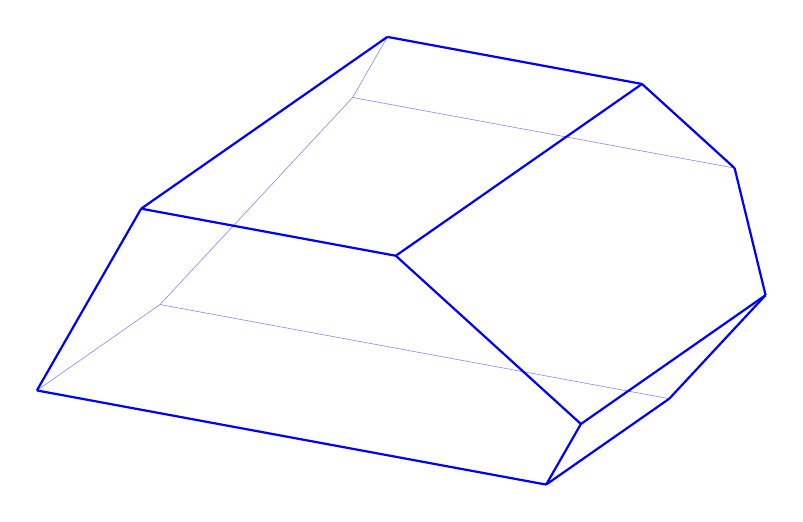
\begin{tikzpicture}%
	[x={(-0.366215cm, -0.789554cm)},
	y={(0.235950cm, -0.590693cm)},
	z={(0.900119cm, -0.166391cm)},
	scale=.550000,
	back/.style={very thin, opacity=0.5},
	edge/.style={color=blue, thick},
	facet/.style={fill=blue,fill opacity=0},
	vertex/.style={}]
%
%
%% This TikZ-picture was produce with Sagemath version 9.5
%% with the command: ._tikz_3d_in_3d and parameters:
%% view = [-481, 324, -815]
%% angle = 141.0
%% scale = 1
%% edge_color = blue
%% facet_color = blue
%% opacity = 0.5
%% vertex_color = blue
%% axis = False

%% Coordinate of the vertices:
%%
\coordinate (-3.33333, 3.77124, 0.00000) at (-3.33333, 3.77124, 0.00000);
\coordinate (-3.33333, 3.77124, 6.53197) at (-3.33333, 3.77124, 6.53197);
\coordinate (-3.33333, 6.59966, -1.63299) at (-3.33333, 6.59966, -1.63299);
\coordinate (-3.33333, 6.59966, 8.16497) at (-3.33333, 6.59966, 8.16497);
\coordinate (-0.66667, 7.54247, 9.79796) at (-0.66667, 7.54247, 9.79796);
\coordinate (2.00000, 8.48528, -4.89898) at (2.00000, 8.48528, -4.89898);
\coordinate (2.00000, 8.48528, 8.16497) at (2.00000, 8.48528, 8.16497);
\coordinate (7.33333, -3.77124, 0.00000) at (7.33333, -3.77124, 0.00000);
\coordinate (7.33333, -3.77124, 6.53197) at (7.33333, -3.77124, 6.53197);
\coordinate (7.33333, 1.88562, 9.79796) at (7.33333, 1.88562, 9.79796);
\coordinate (7.33333, 4.71405, -4.89898) at (7.33333, 4.71405, -4.89898);
\coordinate (7.33333, 4.71405, 8.16497) at (7.33333, 4.71405, 8.16497);
%%
%%
%% Drawing edges in the back
%%
\draw[edge,back] (-3.33333, 3.77124, 0.00000) -- (-3.33333, 6.59966, -1.63299);
\draw[edge,back] (-3.33333, 6.59966, -1.63299) -- (-3.33333, 6.59966, 8.16497);
\draw[edge,back] (-3.33333, 6.59966, -1.63299) -- (2.00000, 8.48528, -4.89898);
\draw[edge,back] (2.00000, 8.48528, -4.89898) -- (2.00000, 8.48528, 8.16497);
\draw[edge,back] (2.00000, 8.48528, -4.89898) -- (7.33333, 4.71405, -4.89898);
%%
%%
%% Drawing vertices in the back
%%
\node[vertex] at (-3.33333, 6.59966, -1.63299)     {};
\node[vertex] at (2.00000, 8.48528, -4.89898)     {};
%%
%%
%% Drawing the facets
%%
\fill[facet] (7.33333, -3.77124, 6.53197) -- (-3.33333, 3.77124, 6.53197) -- (-3.33333, 3.77124, 0.00000) -- (7.33333, -3.77124, 0.00000) -- cycle {};
\fill[facet] (7.33333, 1.88562, 9.79796) -- (-0.66667, 7.54247, 9.79796) -- (-3.33333, 6.59966, 8.16497) -- (-3.33333, 3.77124, 6.53197) -- (7.33333, -3.77124, 6.53197) -- cycle {};
\fill[facet] (7.33333, 4.71405, 8.16497) -- (2.00000, 8.48528, 8.16497) -- (-0.66667, 7.54247, 9.79796) -- (7.33333, 1.88562, 9.79796) -- cycle {};
\fill[facet] (7.33333, 4.71405, 8.16497) -- (7.33333, 1.88562, 9.79796) -- (7.33333, -3.77124, 6.53197) -- (7.33333, -3.77124, 0.00000) -- (7.33333, 4.71405, -4.89898) -- cycle {};
%%
%%
%% Drawing edges in the front
%%
\draw[edge] (-3.33333, 3.77124, 0.00000) -- (-3.33333, 3.77124, 6.53197);
\draw[edge] (-3.33333, 3.77124, 0.00000) -- (7.33333, -3.77124, 0.00000);
\draw[edge] (-3.33333, 3.77124, 6.53197) -- (-3.33333, 6.59966, 8.16497);
\draw[edge] (-3.33333, 3.77124, 6.53197) -- (7.33333, -3.77124, 6.53197);
\draw[edge] (-3.33333, 6.59966, 8.16497) -- (-0.66667, 7.54247, 9.79796);
\draw[edge] (-0.66667, 7.54247, 9.79796) -- (2.00000, 8.48528, 8.16497);
\draw[edge] (-0.66667, 7.54247, 9.79796) -- (7.33333, 1.88562, 9.79796);
\draw[edge] (2.00000, 8.48528, 8.16497) -- (7.33333, 4.71405, 8.16497);
\draw[edge] (7.33333, -3.77124, 0.00000) -- (7.33333, -3.77124, 6.53197);
\draw[edge] (7.33333, -3.77124, 0.00000) -- (7.33333, 4.71405, -4.89898);
\draw[edge] (7.33333, -3.77124, 6.53197) -- (7.33333, 1.88562, 9.79796);
\draw[edge] (7.33333, 1.88562, 9.79796) -- (7.33333, 4.71405, 8.16497);
\draw[edge] (7.33333, 4.71405, -4.89898) -- (7.33333, 4.71405, 8.16497);
%%
%%
%% Drawing the vertices in the front
%%
\node[vertex] at (-3.33333, 3.77124, 0.00000)     {};
\node[vertex] at (-3.33333, 3.77124, 6.53197)     {};
\node[vertex] at (-3.33333, 6.59966, 8.16497)     {};
\node[vertex] at (-0.66667, 7.54247, 9.79796)     {};
\node[vertex] at (2.00000, 8.48528, 8.16497)     {};
\node[vertex] at (7.33333, -3.77124, 0.00000)     {};
\node[vertex] at (7.33333, -3.77124, 6.53197)     {};
\node[vertex] at (7.33333, 1.88562, 9.79796)     {};
\node[vertex] at (7.33333, 4.71405, -4.89898)     {};
\node[vertex] at (7.33333, 4.71405, 8.16497)     {};
%%
%%
\end{tikzpicture}